\documentclass[12pt]{article}
\usepackage[utf8]{inputenc}
\usepackage{graphicx}
\usepackage{geometry}
\usepackage{float}
\usepackage{hyperref}
\usepackage{fancyhdr}
\usepackage{textgreek}

\geometry{
  left=2.5cm,
  right=2.5cm,
  top=2.5cm,
  bottom=2.5cm,
}


\title{Health monitoring system}
\author{}

\newcommand{\members}{\centering  {- BEN SALEM Ahmed} \ \\ \centering {- LABIDI Aymen~~~~~~~~}}

\date{\today}

\newcommand{\faculty}{\centering  {~~~~~~~~~~~~~~- MOHAMED BECHA Kaaniche}}


%------------------------------------------------------------------------
%DO NOT MODIFY ANY OF THE FOLLOWING ITEMS
%------------------------------------------------------------------------
\makeatletter
\let\thetitle\@title
\let\theauthor\@author
\let\thedate\@date
\makeatother


\pagestyle{fancy}
\fancyhf{}
\rhead{\theauthor}
\lhead{\thetitle}
\cfoot{\thepage}

\begin{document}
\begin{titlepage}
	\centering
    \includegraphics[scale = 0.4]{logo.png}\\[3.0 cm]

	\rule{\linewidth}{0.2 mm} \\[0.4 cm]
	{ \huge \bfseries  \centering ~~~~~~Scope statement:
     \newline \centering \thetitle}\\
	\rule{\linewidth}{0.2 mm} \\[1.5 cm]
    
	
	\begin{minipage}{0.8\textwidth}
		\begin{flushleft} \large
			\emph{Authors:}\\
            \members  \\ 
        \end{flushleft}
        \begin{flushleft} \large
        \ \\
            \emph{Faculty Adviser:} \\
            \faculty
	\end{flushleft}
	\end{minipage}
			
	
		
 
	\vfill

\end{titlepage}

\tableofcontents
\pagebreak


\section{Concept}
\subsection{Project context}
Cardiopulmonary disorders, or "Cardiorespiratory Disorders," refer to health conditions where abnormalities in heart and respiratory functions are interconnected, making them interdependent. Two significant diseases within the cardiopulmonary disorders category are Atrial Fibrillation (AFib) and Obstructive Sleep Apnea (OSA). AFib primarily falls under the cardiovascular or heart-related disorder classification as a specific type of arrhythmia within the broader category of heart rhythm disorders. In contrast, OSA is categorized as a sleep disorder, specifically a form of sleep apnea within the domain of sleep-related breathing disorders. Both AFib and OSA are classified under the cardiopulmonary disorders category due to their potential overlap, with one condition capable of influencing the other. Managing and treating such conditions often necessitates a holistic approach that addresses both cardiac and respiratory health.

Cardiorespiratory diseases are the most common cause of death worldwide over the last few decades in developed as well as underdeveloped and developing countries. Early detection of cardiac diseases and continuous supervision of clinicians can reduce the mortality rate. However, accurate detection of heart diseases in all cases and consultation of a patient for 24 hours by a doctor is not available since it requires more sapience, time, and expertise.

\subsection{Problem statement}
\begin{itemize}
    \item How can we develop a system for measuring a person's vital signs such as blood pressure and blood glucose, tracking their health over time, and providing insights and recommendations for maintaining or improving their well-being?
    \item How can we create a solution that effectively identifies advanced health risks and issues in users' vital signs data, providing timely notifications and encouraging them to seek medical advice or lifestyle changes for early intervention and prevention?
\end{itemize}

\subsection{Objectives}
\begin{itemize}
    \item Measure persons' vital Signs.
    \item Predict user's risk level.
    \item Notify user in case of a health concern.
    \item Help the user track their health status.
\end{itemize}
\newpage
\section{Client}
Our potential clients are individuals who are interested in proactive health monitoring, including health-conscious individuals, patients with chronic conditions, seniors, health and wellness professionals. The product could be adjusted so that our client could include healthcare facilities and insurance providers.

\section{Functional need}
\subsection{Sensors and IoT network}
In the IoT system, it is necessary to recognize the person conducting the measurement. This will help us deal with multiple users. A LED indicator should activate to alert the user that the measurement process is underway. The IoT system should enable the user to measure the following parameters:
\begin{itemize}
    \item Heart Rate (HR): is a vital sign that reflects the cardiovascular health of an individual. Variations in heart rate can indicate conditions such as arrhythmias, stress, or physical activity, making it a valuable parameter for assessing overall cardiac well-being. 
    \item Oxygen Saturation (SpO2): Monitoring oxygen saturation is crucial for assessing the efficiency of the respiratory system in delivering oxygen to the body's tissues. Low oxygen saturation can be an early indicator of respiratory issues, sleep apnea, or cardiovascular problems, while maintaining optimal oxygen levels is vital for overall health.
    \item ECG (Electrocardiogram): ECG data provides a detailed analysis of the electrical activity of the heart. It is indispensable for the early detection of arrhythmias, heart diseases, and other cardiac abnormalities. ECG can offer insights into the risk of heart attacks, strokes, and other serious conditions.
    \item Temperature (TEMP): Body temperature is a key indicator of an individual's health status and can help in the early detection of infections, inflammations, or fever, which may be symptoms of various diseases. Monitoring temperature over time can provide valuable information about the body's response to illnesses and potential health risks.
\end{itemize}
A display will show the value of each sensor. The sensors must send the data to the board, which stores them in the Cloud. An alert system is needed to notify the user of the issue (elevated heart rate, low heart rate, elevated temperature, high temperature, elevated oxygen saturation, high oxygen saturation), for a variable duration, and can be disabled by the user.

\subsection{PWA application}
This application will enable the user to:
\begin{itemize}
    \item View the results (graph for ECG, heart rate, and temperature evolution) with an option to choose the period of visualization.
    \item Predict their health status (whether they are healthy or the likelihood of future illness or issues).
    \item Utilize Location-Based Services (LBS) to pinpoint the user's location, enabling us to collect environmental data such as temperature and humidity. This data integration serves to enhance our model by contextualizing the user's temperature readings based on environmental conditions.
    \item In the event of an illness, activate an alert system.
    
\end{itemize}
\section{Machine learning integration}
\subsection{Model development}
The central aim of model development is to construct a machine learning model with the capability to provide precise predictions regarding an individual's risk of having a cardiopulmonary disorder. This predictive model relies on a range of specific health indicators, including heart rate , oxygen saturation, electrocardiogram data, temperature, and the ambient environmental temperature. The intended model output is a risk level score, ranging from 0 to 5,where 0 represent low risk, and 5 represents high risk, with the requirement to attain a minimum accuracy of 95\% while keeping the false positive rate below 0.1\%.
\subsection{MLOps implementation}
This part serves as the backbone for the continuous refinement and operational management of the machine learning model. It encompasses the following key aspects:
\begin{enumerate}
    \item Automated model training and deployment: The MLOps framework will automate the training of the machine learning model using the provided health and environmental data. Once trained, the model will be deployed to ensure real-time predictions and updates.

    \item Continuous monitoring: MLOps tools will continuously monitor the model's performance, assessing its accuracy and identifying any deviations or drift. This monitoring helps ensure that the model remains effective over time.

    \item Alerts and notifications: When the model detects potential cardiopulmonary disorders based on user data, it triggers automated alerts and notifications to users, encouraging them to take timely action and seek medical advice.

    \item Data versioning and tracking: MLOps practices will be employed to manage data versioning and tracking, preserving historical health information for reference and analysis.

    \item Security and compliance: The implementation includes stringent security measures to safeguard user health data, ensuring compliance with data privacy regulations. This involves encryption, access controls, and data anonymization.

    \item Model performance optimization: MLOps will assist in optimizing the model's performance, including hyperparameter tuning and efficient resource allocation, to ensure accurate predictions.

    \item Feedback loop: User feedback will be integrated into the MLOps process to enhance the model's accuracy and its ability to provide relevant and actionable insights.
\end{enumerate}
The MLOps implementation is crucial to maintaining the accuracy, security, and reliability of the cardiopulmonary disorder prediction model, ensuring it evolves to meet the changing needs of users and environmental conditions.

\section{Equipment}
After conducting research, we have identified the following elements as necessary:
\begin{itemize}
    \item Max30102 Pulse sensors: for heart rate and oxygen saturation.
    \item LM35-DZ: Temperature sensor.
    \item AD8232: ECG module.
    \item Raspberry Pi 4 (although Raspberry Pi 3 is also suitable, alternatively, an Arduino and a screen can be used).
    \item A buzzer: for sound.
    \item A LED: for notifications (whatever color).
    \item 1 resistor of 220 Ω.
    \item A camera with a minimum resolution of 160x160 for a distance of 20 cm.
    \item Connecting wires.
\end{itemize}


\section{Technologies choice}
\subsection{Back-end}
\begin{itemize}
    \item MongoDB: A NoSQL document-oriented database used for storing user data. It is practical and easy to use in conjunction with Jakarta EE.
    \item MQTT: A lightweight publish-subscribe network protocol used to communicate sensor data to an MQTT broker in the cloud.
\end{itemize}

\subsection{Middleware}
\begin{itemize}
    \item JAX-RS: Java API for RESTful Web Services is a Java programming interface for creating web services with a REST architecture.
    \item WildFly: WildFly, formerly known as JBoss Application Server or JBoss, is a free and open-source Java EE application server written in Java and released under the GNU LGPL license. It can be used on any operating system that provides a Java virtual machine.
    \item Mosquitto: Mosquitto is a widely used MQTT broker, serving as an intermediary for efficient and reliable messaging between IoT devices and the back-end system.
\end{itemize}
\subsection{Front-End}
\begin{itemize}
    \item PWA (Progressive Web App): A PWA is a cross-platform web application that provides a native-like experience to users. It allows you to develop applications for multiple platforms using web technologies like HTML, CSS, and JavaScript. PWAs are easy and quick to code and do not require prior web development knowledge.
\end{itemize}
\subsection{Iot integration}
\begin{itemize}
    \item Flogo: Flogo is an open-source project designed for creating lightweight, event-driven microservices and workflows, making it suitable for orchestrating data flows, data preprocessing, and automation in IoT scenarios.
\end{itemize}
\subsection{MLOPS integration}
In our MLOps integration, we harness a suite of technologies to streamline the operational management of machine learning models, ensuring their continuous accuracy and reliability. Key technology components include:
\begin{enumerate}
\item CI/CD Pipeline: Our continuous integration and continuous deployment (CI/CD) pipeline, powered by Jenkins, is at the core of our MLOps strategy. 

\item Testing technologies: For model validation and data quality assurance, we employ PyTest and Selenium. These testing frameworks aid in verifying the functionality and reliability of our health monitoring system, ensuring that user data is processed accurately.

\item Development technologies: We leverage Python and Jupyter Notebook for model development and experimentation. These technologies provide a versatile and data-centric environment for creating and fine-tuning our machine learning models.

\item Monitoring and logging: Our system relies on Prometheus and Grafana for monitoring and logging. These tools allow us to track the performance of our machine learning models and detect any anomalies, ensuring their continued effectiveness.

\item Data management: MongoDB serves as our database technology, providing a robust and flexible solution for storing and managing user data, health records, and environmental information.
\item Security measures: To safeguard sensitive user data, we implement encryption and access control using HashiCorp Vault.
\item Containerization: Docker containers are used for efficient deployment and scaling, ensuring consistency and ease of management in our system.
\item Stream processing: Apache Kafka is employed to handle real-time data streams from sensors, enabling timely updates and notifications in our health monitoring system.

\end{enumerate}


\section{Architecture}
\begin{figure}[H]
    \centering
    \includegraphics[width=0.8\textwidth]{archi.png}
    \caption{Architecture}
    \label{fig:architecture}
\end{figure}
The diagram above describes the main architecture of the Health monitoring system which is mainly composed by Backend, Middleware and Frontend.
\section{Deployment diagram}
\begin{figure}[H]
    \centering
    \includegraphics[width=1.\textwidth]{dep.png}
    \caption{Deployment Diagram}
    \label{fig:Deployment Diagram}
\end{figure}

\section{Timeline and tasks}
\begin{figure}[H]
    \centering
    \includegraphics[width=1.\textwidth]{WEEK1.png}
    \caption{Gantt Diagram.}
    \label{fig:Gantt}
\end{figure}
\newpage
The Gantt diagram, which enables the project's progress to be graphically represented, is shown in the explanation above. It makes it possible to visually illustrate the project's progress and the length of each process.


\section{Methodology}
Throughout the project, we will be utilizing Extreme Programming (XP), an Agile software development framework renowned for its commitment to delivering superior software quality and enhancing the personal satisfaction of the development team. This methodology is exceptionally well-suited to our project due to its adaptability, specifically tailored for short-duration projects where last-minute requirement changes are common.

\subsection{Principles}
XP's principles align with those of agile methodologies but are distinguished by their extreme emphasis. XP is founded on:
\begin{itemize}
    \item High responsiveness to changing customer needs.
    \item Teamwork, in our context represented by Pair Programming.
    \item Delivering high-quality work.
    \item Early, high-quality testing.
\end{itemize}

\subsection{Process}
The XP framework normally involves 5 phases or stages of the development process that iterate continuously:
\begin{enumerate}
    \item Planning: In the initial stage, we create our own user stories and define the desired outcomes. Requirements are provided, and we estimate the stories, creating a release plan that breaks the project into iterations to cover the required functionality incrementally. If certain stories cannot be accurately estimated, we introduce "spikes," indicating that further research is necessary.
    \item Design: While designing is an integral part of the planning process, it is essential enough to be highlighted separately. It is closely tied to one of the core XP values we will discuss later – simplicity. A well-thought-out design brings logical structure to the system, helping us avoid unnecessary complexities and redundancies.
    \item Coding: This phase involves the actual implementation of code, and it follows specific XP practices, including adherence to coding standards, pair programming, continuous integration, and collective code ownership.
    \item Testing: Testing is at the heart of Extreme Programming. It is an ongoing activity encompassing both unit tests, which are automated tests that verify the proper functioning of individual features, and acceptance tests, where customers assess whether the system aligns with the initial requirements.
    \item Listening: Listening emphasizes continuous communication and feedback. Coaches and project managers play a pivotal role in conveying the business logic and expected value to the team, ensuring a shared understanding of the project's goals and requirements.
\end{enumerate}

\begin{figure}[H]
    \centering
    \includegraphics[width=0.85\textwidth]{pipe.png}
    \caption{Extreme programming life-cycle}
    \label{fig:XP}
\end{figure}

\section{Limitations}
As we embark on the development of our healthcare monitoring system, it's important to anticipate and address various challenges that may arise during its implementation.
\begin{itemize}
    \item Internet Connectivity Interruptions: One limitation lies in the reliance on internet connectivity. In cases of internet outages, real-time monitoring and user alerts for critical health changes may not be achievable.
    \item Sensor Data Accuracy: There's the possibility of false alarms due to inaccuracies in sensor data or anomalies detected by the algorithm, potentially causing unnecessary concerns for users.
    \item Proximity of IoT Devices: The correct identification of health data may be affected by the proximity of IoT devices to each other. If IoT devices are placed very closely, they might detect changes in neighboring devices, impacting the accuracy of the data.
    \item Sensor Placement and Thresholds: Placing the IoT sensors correctly is critical. Inaccurate placement or poorly defined thresholds for measured metrics may lead to misinterpretations and unnecessary alerts.
    \item Data Volume and Processing: Handling a large volume of health data generated by multiple users and devices can be challenging. Processing and analyzing this data efficiently is essential for providing real-time insights.
\end{itemize}
\section{Business study}
The Business Study section provides an overall view of our project's business model and marketing policy.

\subsection{Business Model Canvas (BMC)}
The Business Model Canvas serves as a visual representation of our project's main aspects, such as value proposition, customer segmentation, channels, cost structure, revenue stream, and more. The BMC is depicted in the figure below:

\begin{figure}[H]
    \centering
    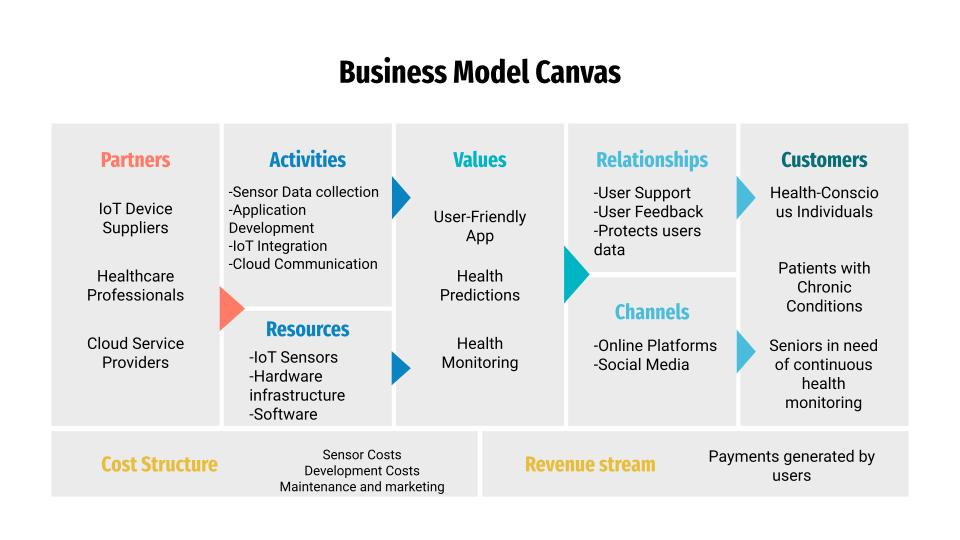
\includegraphics[width=1.\textwidth]{bmc.jpg}
    \caption{Business Model Canvas}
    \label{fig:bmc}
\end{figure}

\subsection{Marketing policy}
Our marketing policy is focused on delivering value to our customers while maintaining a strong market presence. It encompasses the following aspects:

\subsubsection{Product}
\begin{itemize}
    \item A sophisticated IoT component architecture for seamless health monitoring.
    \item Efficient management of health monitoring with mobile applications.
    \item Integration of Location-Based Services (LBS) to deliver precise health insights.
    \item Continuous algorithm improvement through MLOps for enhanced accuracy.
    

\end{itemize}
\subsubsection{Price}
\begin{itemize}
    \item Competitive pricing with customizable rates to suit individual users and healthcare institutions.
    \item Assurance of warranty and after-sales service.
\end{itemize}
\subsubsection{Promotion}
\begin{itemize}
    \item We use a multi-channel approach for promotion, including digital marketing, partnerships with healthcare providers, and user referrals.
    \item Collaborative advertising with our trusted partners to expand our reach and impact.

\end{itemize}
\subsubsection{Place}
\begin{itemize}
    \item Our services are accessible through web platforms and mobile applications, making it convenient for users to access health monitoring.
\end{itemize}

\section{Deliverables}
\begin{itemize}
    \item Conceptual Document: This document presents in a detailed and structured manner the specifications and the services to be provided.
    \item Source code of the various project components on GitHub
    \item Prototype/simulation of the intelligent healthcare monitoring system.
    \item Demonstration Video: An mp4 format video that contains a demonstration of the proposed solution.
\end{itemize}

\end{document}
